% Chapter 1

\chapter{Result} % Main chapter title

\label{Chapter2} % For referencing the chapter elsewhere, use \ref{Chapter1} 

%----------------------------------------------------------------------------------------

\section{Run1 (20170109-2017012; KEK)}
\subsection{Member}
Yuki, Cory, Bin-Hua, Takaaki, Takahiro
\subsection{Test setup}
\begin{figure}
	\begin{center}
                 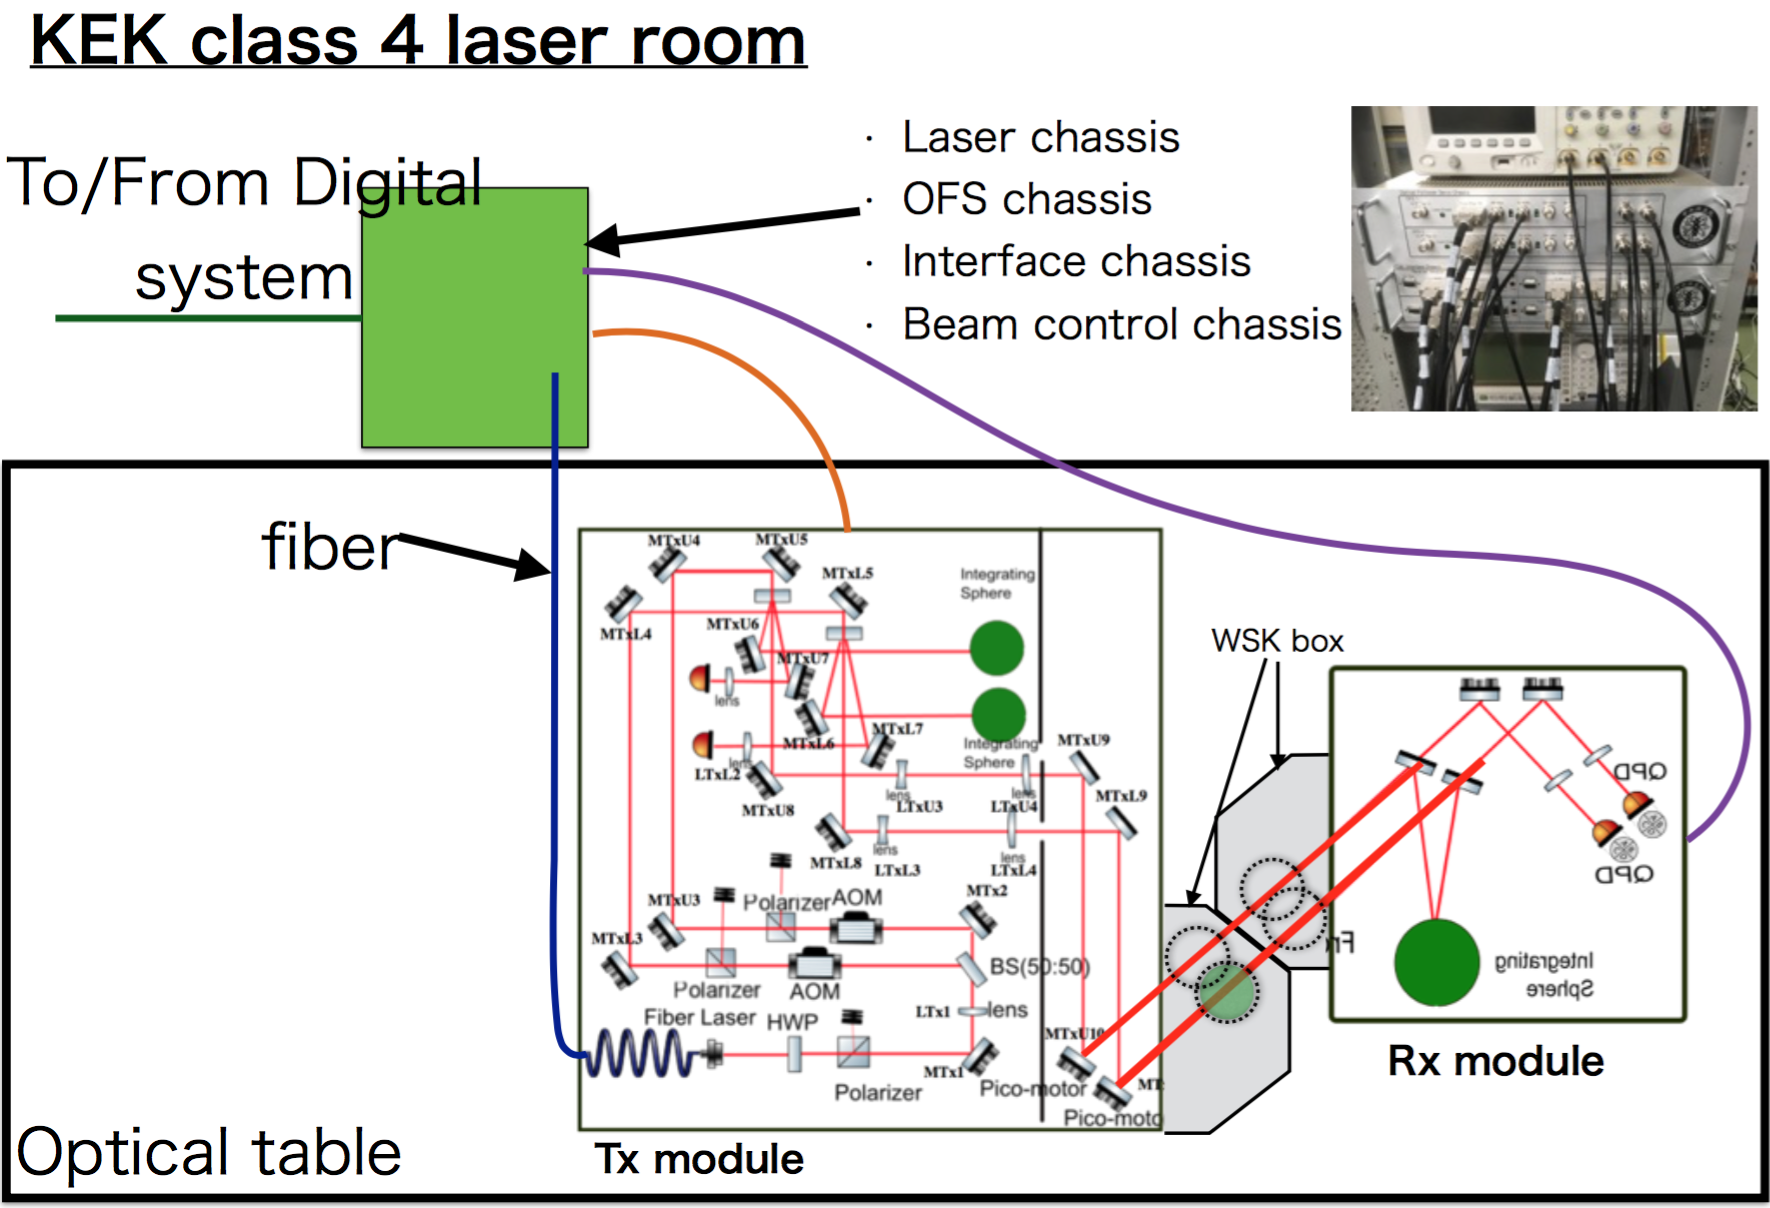
\includegraphics[width=15cm]{Setup_170109.eps}
                 \caption{Setup of the integration test} 
                 \label{fig:Setup} 
	\end{center}
\end{figure}
\subsection{Log: 01\/09}
Main goal of Jan. 9th measurement is noise debugging.
In previous measurement, the measured noise is larger than that of requirement.
To reduce the noise, we tried the following things:
\paragraph{Open loop gain}


\subsection{Injection Test}
\subsubsection{Time delay measurement}

To investigate the time delay of PCal system, we injected some Sine-Gaussian signal.
 Sine-Gaussian signal for our injection test is defined as Eq.~\ref{eq:singaussian}
\begin{equation}
\label{eq:singaussian}
    A \exp\left(-\frac{(t-t_0)^2}{\tau^2}\right) \cos ( 2 \pi f_0 (t-t_0))
\end{equation}
\begin{equation*}
   \tau = \frac{Q}{ \sqrt{2} \pi f_0}
\end{equation*}



% Requires the booktabs if the memoir class is not being used
\begin{table}[htbp]
   \centering
   %\topcaption{Table captions are better up top} % requires the topcapt package
   \begin{tabular}{ rrcc } % Column formatting, @{} suppresses leading/trailing space
      \toprule
%      \multicolumn{2}{c}{Item} \\
%      \cmidrule(r){1-2} % Partial rule. (r) trims the line a little bit on the right; (l) & (lr) also possible
      $A$ (Volts)   & $f_0$ (Hz) & Injected GPS Time (~$t_0-10$ s~) & OFS\_PD GPS Time (s) \\
      \midrule
        1 & 7 & 13.65  \\
        1 & 35      &  &\\
        1 & 330     &   &\\
        1 & 1k      &   &\\
        1 & 3k      &   &\\
      \bottomrule
   \end{tabular}
   \caption{Time delay measurement results}
   \label{tab:timedelay}
\end{table}




\section{Run2 (201702; Toyama)}

\section{Run3 (201703; KAGRA Y-end)}
%----------------------------------------------------------------------------------------

